% !Mode:: "TeX:UTF-8" 

\BiChapter{SDN硬件流表可扩展性研究}{the table resource of SDN}


\BiSection{本章引论}{aa}



\BiSection{背景}{aa}

软件定义网络的实时标准为OpenFlow协议,其将网络解耦为控制平面和数据平面。控制平面内可运行网络操作系统,所有传统的网络转发功能都可以由操作系统内应用来完成。网络管理人员只需要开发网络应用即可管理网络内所有设备的行为,通常应用具有标准的通信接口,可支持各类高级语言,且运行环境单一且标准,屏蔽了过去由于设备数量众多导致的开发流程复杂等问题。OpenFlow交换机是支持软件定义网络的标准化设备,负责SDN网络内数据平面内数据包转发操作。OpenFlow交换机支持统一的南向协议,并与控制器通信传递配置信息与数据层状态。

目前高速数据包处理设备性能需求可达数十个Tbps,因此交换机内部需要使用基于硬件的高速缓存(如,TCAM,SRAM等)来进行查表操作。带有掩码功能的查找表(TCAM)是做IP最长前缀查找的高性能核心部件。TCAM具有单周期吞吐的流水线掩码查找能力使得其功能难以由一般存储器代替。但其价格以及能源消耗都较大,基于TCAM的流表容量通常都比较小,且极有溢出的可能。数据包在数据平面中被流表匹配,并得到相应的执行指令,待由后续机构处理。若数据包在流表中没有被成功匹配,则被称作Table-Miss(未匹配)现象。一般未匹配现象的处理方式为丢包,但在OpenFlow协议中支持了reactive处理模式,为后续数据包成功处理,将数据包实时发给控制器,等待控制器处理结果并下发新的可匹配此流的表项。

流表溢出会导致交换机转发性能大幅降低,甚至会导致数据平面与控制器通信报文数量爆炸,给SDN控制器的安全造成隐患\citeup{qsy2018openflow}。网络当中流量变化异常迅速,为减小Table-Miss事件,交换机须能够进行快速流表更新或大容量查找。拥有无限大容量的查找表可以将所有可能出现的流,都预先存储下来。但显然不现实,因此提高流表更新速率成为交换设备的一个硬指标,目前商用交换机的流表更新速度不超过10000条/秒。
基于TCAM的流表删除和添加操作比较复杂,且TCAM有效容量有限,这为设计人员继续增强性能提出了很大难题。

在解决此类问题时,研究人员通常从以下两方面着手:(1)提升流表项数量。当TCAM存储容量固定时,假设宽度为key、深度为depth,二者的乘积恒定。显然如果可以降低流表项宽度值key,可以变相增加流表项数量。在数据中心网络场景下,可以通过重新定义包头域宽度来定义流,无需使用现有过宽的包头域。例如工作\citeup{kannan2013compact}将所有流映射到16bits宽度的匹配域,可增加流表项容量10倍左右,等数据包离开网关时在将原始包头还原。但这种思路仅仅在内网有效,而应对如今更大流量的骨干网,核心网显然无所适从。(2)




\BiSection{基于流量特征的问题分析}{aa}

本文通过分析真实流量特征,来证明单纯地依靠增加流表容量无法完全避免流表溢出现象。本文分析ISP服务供应商给出的一段真实数据(新西兰,15分钟,2千万个数据包),发现增大流表容量的确可以减少流表的更新速率。如图\ref{fig:ftsupdate}本文使用最近最少使用(Least Recently Used,LRU)替代算法,当设置流表容量为一万条时,流量变化超过交换机更新极限的情况大约占到10\%。若进一步增大到5万条,约有6\%的流量会引发流表溢出。再将流表容量扩大到25万条,仍有4\%的流量无法得到及时地更新。

\begin{figure}[!ht]
	\centering 
	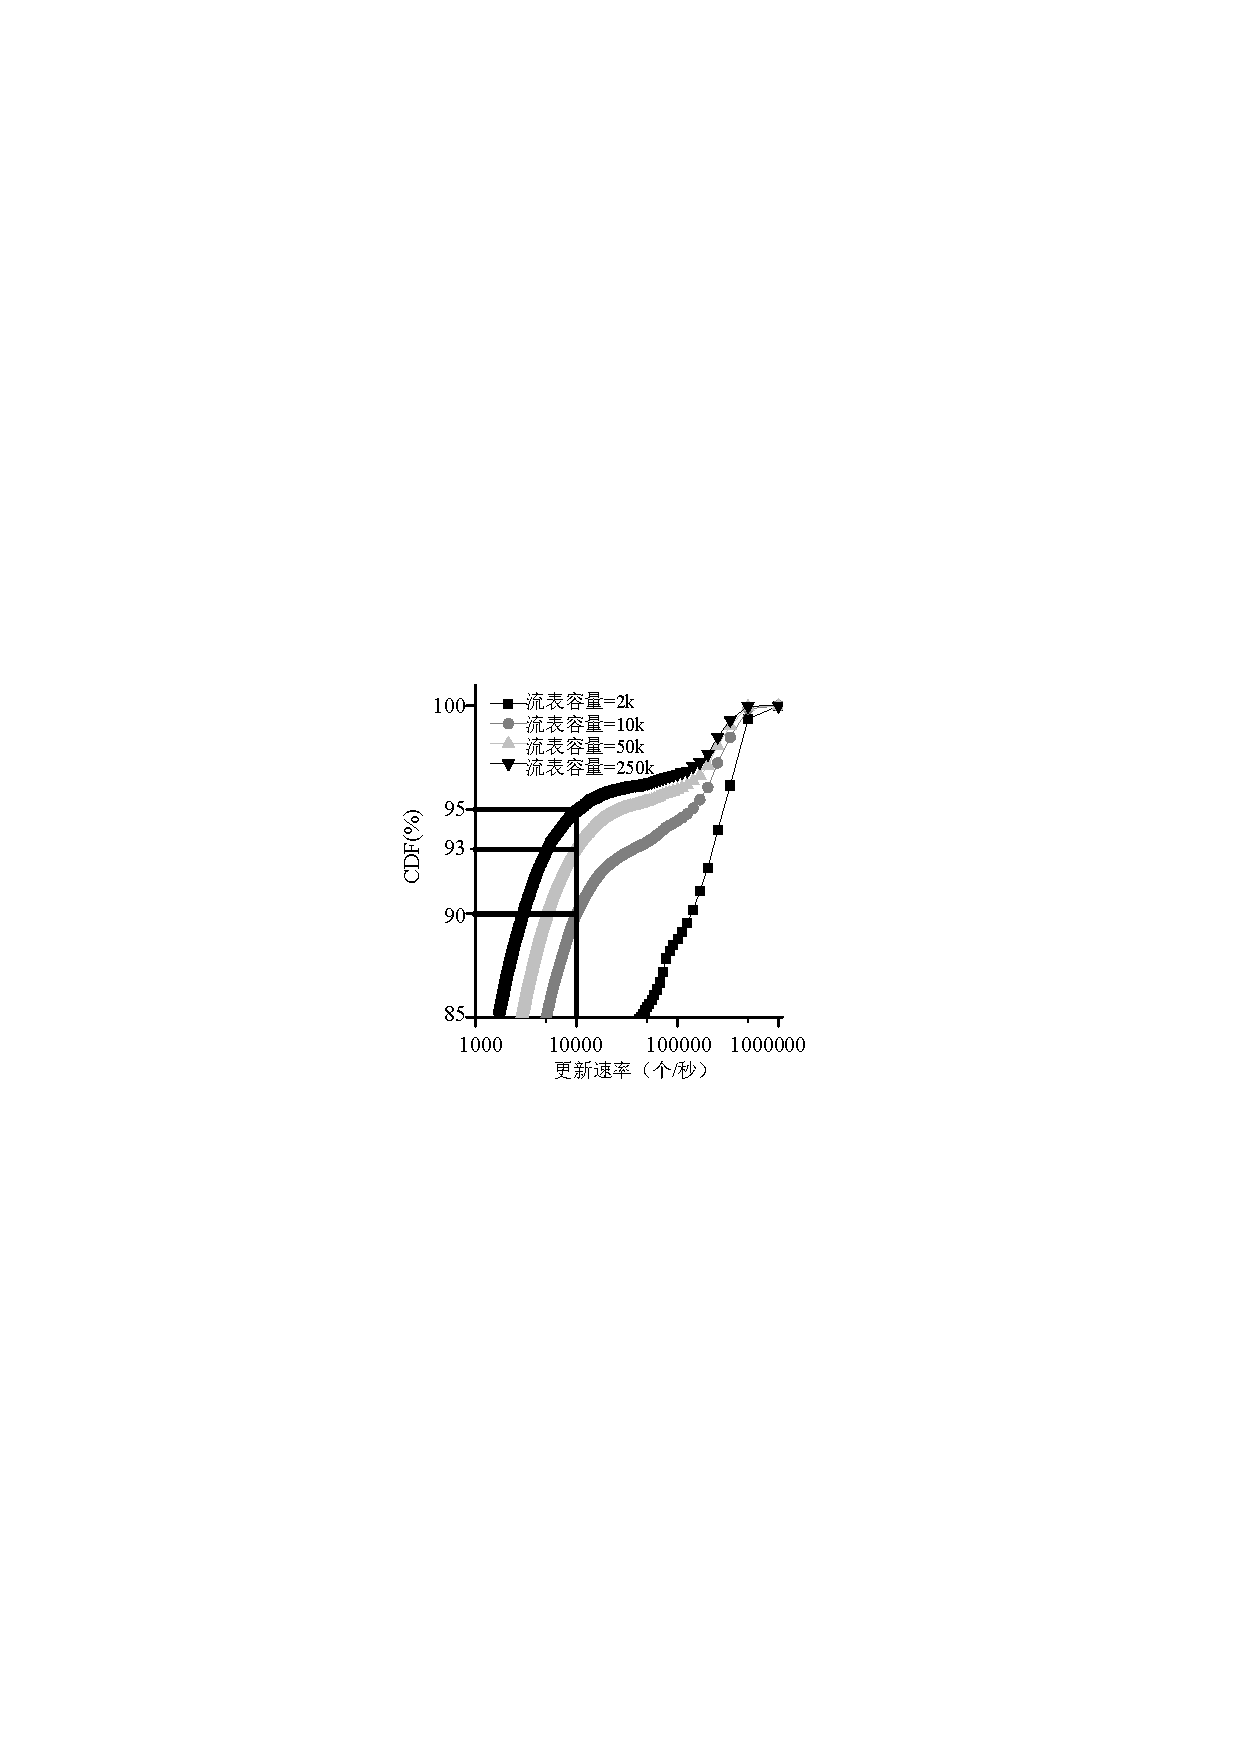
\includegraphics[scale=1]{ftsupdate.pdf}
	\caption{流量更新速率的概率累计分布} \label{fig:ftsupdate}
\end{figure}

根据Openf协议,流表最大支持45个域(144Bytes),流表资源消耗量大的情况在OpenFlow交换机中尤为凸显。面对上述问题,为使SDN的技术优势在广域网间应用,业界不得不使用以及购买性能更强价格更昂贵的交换机。在实际应用中,若交换机流表资源不足,对于最终无法更新的流,交换机会将他们按照Table-Miss策略处理。目前的控制策略大都会以Packet-In消息的方式上报给控制器。若Packet-In消息数目过多,会引起安全通道传输阻塞以及引发控制器处理阻塞,不但会引发控制器安全问题,且影响到其他服务,会加剧数据平面转发效率下降。

\BiSection{流表共享机制}{aa}




\BiSection{基于OpenFlow交换机的随机路由策略}{aa}



\BiSection{系统评估}{aa}



\BiSection{本章小结}{aa}
